\documentclass[border=10pt]{standalone}

\usepackage{tikz}
\usepackage{tikzsymbols}
\usetikzlibrary{calc,patterns,shapes.geometric}

\def\centerarc[#1](#2)(#3:#4:#5){\draw[#1] ($(#2)+({#5*cos(#3)},{#5*sin(#3)})$) arc (#3:#4:#5);}

\begin{document}
	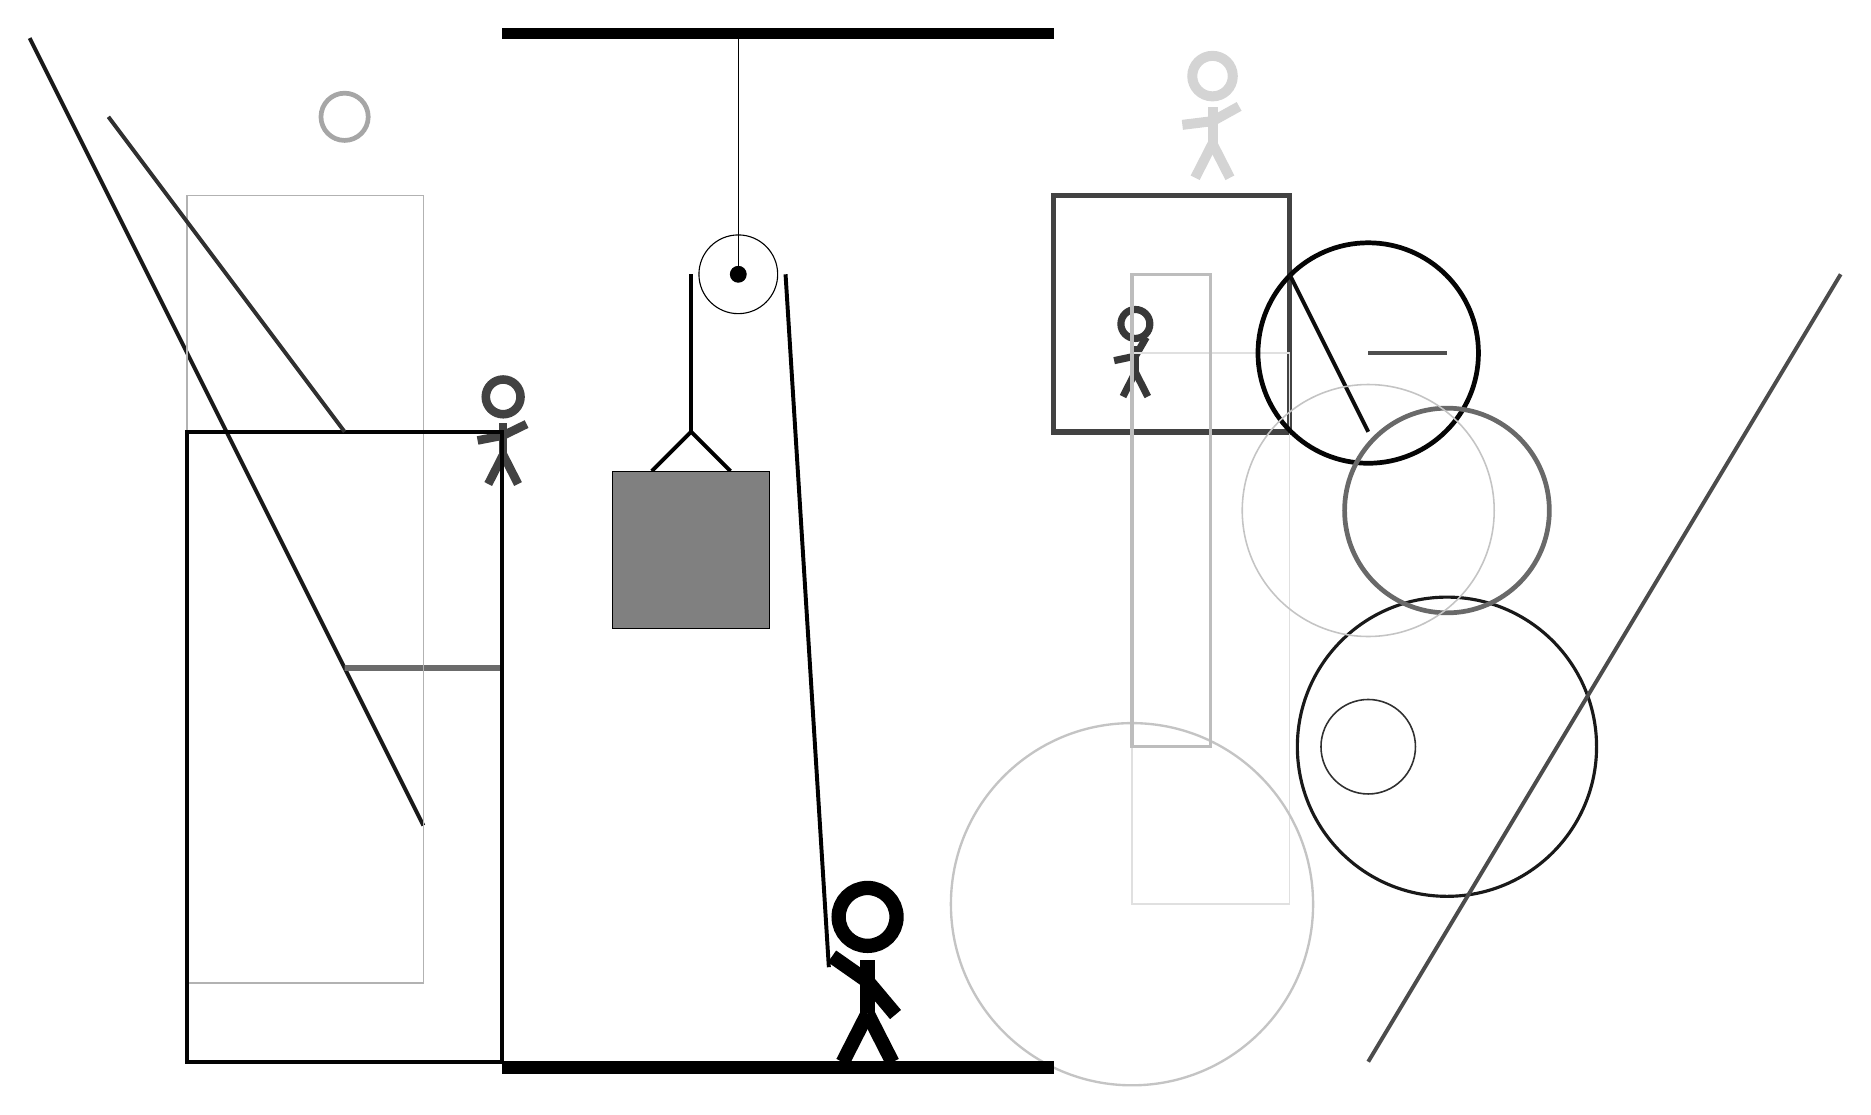
\begin{tikzpicture}
		%%%%% START %%%%%
		
		\draw[fill=black] (-2, 10) rectangle (5, 10.125);
		
		\draw[line width=0.7mm, color=black!74] (5, 8) rectangle (8, 5);
		
		\draw [line width=0.4mm, color=black!90](10, 1) circle (1.9);
		\draw[line width=0.5mm, color=black!90](-3, 0) -- (-8, 10);
		\draw[line width=0.7mm, color=black!58] (-2, 2) rectangle (-4, 2);
		\draw[line width=0.2mm, color=black!30] (-3, -2) rectangle (-6, 8);
		
		\draw [line width=0.6mm, color=black!35](-4, 9) circle (0.3);
		\draw[line width=0.5mm, color=black!69](9, 6) -- (10, 6);
		\node[line width=0.4mm, color=black!78] at (6, 6) {\Strichmaxerl[5][12][60]};
		\node[line width=0.7mm, color=black!74] at (-2, 5) {\Strichmaxerl[6][11][26]};
		
		\draw[line width=0.2mm, color=black!12] (6, -1) rectangle (8, 6);
		\draw[line width=0.5mm, color=black!99] (-2, -3) rectangle (-6, 5);
		\draw [line width=0.6mm, color=black!98](9, 6) circle (1.4);
		\draw [line width=0.2mm, color=black!81](9, 1) circle (0.6);
		
		\draw [line width=0.6mm, color=black!59](10, 4) circle (1.3);
		\draw [line width=0.3mm, color=black!23](6, -1) circle (2.3);
		\node[line width=0.3mm, color=black!17] at (7, 9) {\Strichmaxerl[7][7][29]};
		
		\draw[line width=0.5mm, color=black!70](9, -3) -- (15, 7);
		
		\draw[line width=0.5mm, color=black!95](9, 5) -- (8, 7);
		\draw[line width=0.5mm, color=black!81](-7, 9) -- (-4, 5);
		
		\draw[line width=0.4mm, color=black!26] (7, 1) rectangle (6, 7);
		\draw [line width=0.2mm, color=black!23](9, 4) circle (1.6);
		
		
		\draw (1, 7) circle (0.5);
		\draw[fill=black] (1, 7) circle (0.1);
		\draw (1, 10) -- (1, 7);
		
		\draw[line width=0.5mm] (-0.1, 4.5) -- (0.4, 5.0) -- (0.9, 4.5);
		\draw[fill=black!50] (-0.6, 4.5) rectangle (1.4, 2.5);
		
		\draw[line width=0.5mm] (0.4, 7) -- (0.4, 5.0);
		\centerarc[line width=0.5mm](1, 7)(0:180:0.6);
		\draw[line width=0.5mm](1.6, 7) -- (2.15, -1.8);
		
		\node at (2.6, -1.9) {\Strichmaxerl[10][-35][-50]};
		
		\draw[fill=black] (-2, -3) rectangle (5, -3.15);
		
		%%%%% END %%%%%
	\end{tikzpicture}
\end{document}